\documentclass{article}
\usepackage[utf8]{inputenc}
\usepackage{amsmath}
\usepackage{amsfonts}
\usepackage{amssymb}
\usepackage{graphicx}
\usepackage[colorlinks=true, allcolors=blue]{hyperref}
\usepackage{geometry}
\geometry{a4paper, margin=1in}
\usepackage{titlesec}
\usepackage{float}
\usepackage{caption}
\usepackage{multicol}


\titleformat{\section}{\Large\bfseries}{}{0em}{\arabic{section}.\ }
\titleformat{\subsection}{\large\bfseries}{}{0em}{\arabic{section}.\arabic{subsection}.\ }
\titleformat{\subsubsection}{\bfseries}{}{0em}{\arabic{section}.\arabic{subsection}.\arabic{subsubsection}.\ }

\begin{document}

\title{\textbf{Comprehensive Report: T-shirt Image Retrieval and Captioning System}}
\author{Mahla Entezari}
\date{January 2025}


\maketitle



\begin{abstract}
This report details the design, implementation, and evaluation of a comprehensive T-shirt image retrieval and captioning system. Leveraging state-of-the-art pre-trained deep learning models from the Hugging Face ecosystem, the system addresses key challenges in multimodal information retrieval. It encompasses three core modules: text-to-image retrieval using CLIP and FAISS for efficient similarity search; automated image captioning using BLIP for generating descriptive textual metadata; and text-to-text retrieval based on these generated captions. The project emphasizes the practical application of pre-trained models to build robust AI solutions without the need for extensive training from scratch. The report provides a thorough explanation of the methodology, model justifications, system implementation, and a qualitative assessment of the results, concluding with limitations and future directions for enhancement and scalability.
\end{abstract}

\newpage
\tableofcontents
\newpage


%\begin{multicols}{2}


\section{Introduction to Multimodal Information Retrieval}
\label{sec:introduction}



The rapidly expanding volume of digital content necessitates advanced methods for efficient information retrieval. While traditional retrieval systems often rely on single modalities, such as text-based search for documents or metadata-driven search for images, the true value of modern data often lies in its \textbf{multimodal nature}. Images are not merely visual data; they often come with associated text (captions, descriptions, tags), or their content can be best understood through textual interpretation. This project delves into the exciting field of multimodal information retrieval, specifically focusing on building a robust system for T-shirt images. The primary objective is to enable users to search for T-shirts using natural language queries and to automatically generate descriptive text for these visual assets.

The increasing availability of large, pre-trained deep learning models has revolutionized the development of such systems. These models, often trained on vast and diverse datasets, have learned powerful representations of both visual and textual information, capable of understanding complex semantic relationships. Leveraging these pre-trained models eliminates the need for extensive data collection and model training from scratch, significantly reducing development time and computational resources. This project strictly adheres to the principle of utilizing pre-trained models from the Hugging Face ecosystem, showcasing their immediate applicability to real-world tasks.

The system is compartmentalized into three interconnected modules:
\begin{itemize}
    \item \textbf{Image Retrieval (Text-to-Image)}: This module allows users to provide a textual query (e.g., "blue graphic T-shirt") and receive the most semantically similar T-shirt images from a dataset of 1,993 images. This task explores contrastive learning principles and the direct application of pre-trained vision-language models for cross-modal similarity.
    \item \textbf{Image Captioning}: This module extends the system's capabilities by generating detailed textual descriptions for each T-shirt image. These machine-generated captions serve as valuable metadata, enriching the images with linguistic context.
    \item \textbf{Text Retrieval (Text-to-Text via Captions)}: Building upon the generated captions, this module enables a more refined text-based search. Given a textual query, the system retrieves images by identifying captions that are most relevant to the query. This involves leveraging text embedding models and similarity computation techniques.
\end{itemize}
This report will systematically detail the methodology, implementation, and results for each of these sub-projects. It will include comprehensive documentation, justification for the chosen pre-trained models, and conceptual standalone inference pipelines to demonstrate the system's capabilities. The overarching goal is to provide a practical understanding of multimodal IR and the immense potential of pre-trained models in bridging the gap between language and vision.

\section{Dataset Description: T-shirt Image Collection}
\label{sec:dataset}


\subsection{Overview and Source}
The dataset central to this project comprises a collection of T-shirt images, specifically provided for hands-on experience in information retrieval. The dataset's focused nature on a single product category (\textbf{T-shirts}) allows for a deep dive into visual and textual characteristics pertinent to e-commerce or fashion applications.

\subsection{Data Volume and Composition}
The dataset consists of \textbf{1,993 distinct T-shirt images}. Each image is a visual representation of a T-shirt, potentially featuring various colors, patterns, designs, graphics, and styles. The images are typically in standard image formats such as JPG, PNG, or JPEG.

\subsection{Key Characteristics Relevant to Information Retrieval}
\begin{itemize}
    \item \textbf{Homogeneous Product Category}: All images belong to the same product category (T-shirts). This homogeneity can simplify some aspects of modeling (e.g., general object recognition is not the primary challenge) but highlights the need for models to distinguish subtle variations within the category (e.g., different types of graphics, shades of color, fabric textures).
    \item \textbf{Absence of Explicit Metadata}: Critically, the provided dataset of 1,993 images does not come with pre-existing textual metadata such as product descriptions, tags, or manual captions. This absence directly motivates the image captioning task, where the system must generate this information automatically, and the text retrieval task, which then leverages these generated captions.
    \item \textbf{Variety in Visual Attributes}: Despite being a single product category, T-shirts can exhibit a wide array of visual attributes:
    \begin{itemize}
        \item \textbf{Colors}: From basic black and white to vibrant hues, pastels, and multi-color combinations.
        \item \textbf{Patterns/Graphics}: Solid, striped, polka-dotted, abstract art, band logos, cartoon characters, text-based graphics, etc.
        \item \textbf{Style}: Crew neck, V-neck, long sleeve, short sleeve, sleeveless, fitted, oversized, etc.
        \item \textbf{Texture}: Cotton, polyester, blended fabrics (though visual distinction might be subtle).
    \end{itemize}
    \item \textbf{Image Quality and Consistency}: While the exact characteristics vary, a typical dataset of this nature would exhibit reasonable image quality, though consistency in background, lighting, and T-shirt presentation (e.g., on a model, flat lay) might fluctuate. Preprocessing steps are essential to standardize inputs for deep learning models.
    \item \textbf{Scalability Consideration}: While 1,993 images is a manageable size for initial experimentation, any practical image retrieval system needs to consider scalability to millions or billions of items. The choice of embedding models and indexing strategies (like FAISS) is crucial for this.
\end{itemize}
The clean nature of the image files, without immediate concerns of corruption or highly irregular formats, provides a solid foundation for directly applying state-of-the-art computer vision and natural language processing techniques. The challenge lies in extracting meaningful, searchable features and descriptions from this purely visual input.

\section{Methodology}
\label{sec:methodology}


My methodology for developing this multimodal information retrieval system for T-shirt images is structured into distinct, yet interconnected, phases. Each phase leverages pre-trained models from Hugging Face, adhering to the project's core constraint of avoiding model training from scratch.

\subsection{Data Loading and Preparation}
\begin{itemize}
    \item \textbf{Image Collection}: The first step involves gathering all 1,993 T-shirt image files from the designated dataset path. The file names are extracted to serve as unique identifiers and pointers to the image data.
    \item \textbf{Image Preprocessing for Models}: Different pre-trained models often have specific input requirements (e.g., image resolution, normalization parameters).
    \begin{itemize}
        \item For CLIP (Image Encoder), images are resized to \textbf{224x224 pixels} and normalized using a specific mean and standard deviation derived from its training data. This ensures consistency with the model's learned representations.
        \item For BLIP (Image Captioning), the model's own processor handles the internal resizing and normalization, abstracting away these details for the user.
    \end{itemize}
    Images are consistently converted to \textbf{RGB format} to ensure uniformity.
\end{itemize}

\subsection{Image Retrieval (Text-to-Image)}
This task focuses on retrieving visually similar T-shirts given a textual query.

\subsubsection{Feature Extraction (Image Embeddings)}
\begin{itemize}
    \item \textbf{Model Selection}: The \texttt{openai/clip-vit-base-patch32} model is chosen for its ability to learn a joint embedding space for images and text.
    \item \textbf{Process}: For each of the 1,993 T-shirt images, the preprocessed image is fed into CLIP's image encoder. The output is a fixed-size, high-dimensional vector (e.g., \textbf{512-dimensional} for base-patch32) that semantically represents the image. This process is performed offline and once to create a searchable database of image features.
    \item \textbf{Storage}: These image embeddings, along with their corresponding image file paths, are stored in memory or persisted to disk (e.g., as NumPy arrays or JSON files).
\end{itemize}

\subsubsection{Indexing for Efficient Search (FAISS)}
To enable rapid nearest-neighbor search over the collection of image embeddings, a \textbf{FAISS} (Facebook AI Similarity Search) index is employed.
\begin{itemize}
    \item \textbf{Index Type}: A \texttt{faiss.IndexFlatL2} index is initialized. This index performs a brute-force L2 (Euclidean) distance search, guaranteeing exact nearest neighbors. For larger datasets, approximate nearest neighbor (ANN) indices would be considered.
    \item \textbf{Adding Embeddings}: The pre-computed image embeddings are added to the FAISS index, making them searchable. This indexing process is also performed offline.
\end{itemize}

\subsubsection{Query Processing and Retrieval}
\begin{itemize}
    \item \textbf{Text Embedding}: When a user inputs a textual query (e.g., "blue graphic T-shirt"), CLIP's text encoder is used to transform this query into a corresponding fixed-size text embedding within the same joint embedding space.
    \item \textbf{Similarity Search}: The query's text embedding is then used to query the FAISS index. FAISS returns the \texttt{top\_k} most similar image embeddings (based on L2 distance) and their original indices in the dataset.
    \item \textbf{Result Presentation}: The images corresponding to these \texttt{top\_k} indices are retrieved from their file paths and displayed to the user, providing a visual representation of the retrieval results.
\end{itemize}

\subsection{Image Captioning}
This task involves generating descriptive textual captions for the T-shirt images.

\subsubsection{Captioning Model Selection}
\begin{itemize}
    \item \textbf{Model}: The \texttt{Salesforce/blip-image-captioning-base} model is chosen. BLIP is a powerful Vision-Language Model capable of generating coherent and contextually relevant captions.
\end{itemize}

\subsubsection{Caption Generation Process}
\begin{itemize}
    \item For each T-shirt image, the image is passed through the BLIP model's processor and then its conditional generation component.
    \item The model outputs a sequence of tokens, which are then decoded back into a human-readable string, forming the image caption.
    \item This process is typically performed offline for all images to pre-compute captions.
    \item \textbf{Caption Storage}: The generated captions are stored in a structured format (e.g., a dictionary mapping image paths to captions, saved as a JSON file) for easy access in subsequent tasks.
\end{itemize}

\subsection{Text Retrieval (Text-to-Text via Captions)}
This task enhances retrieval by leveraging the generated captions.

\subsubsection{Text Embedding (Captions and Query)}
\begin{itemize}
    \item \textbf{Model Reuse}: CLIP (\texttt{openai/clip-vit-base-patch32}) is reused for its text encoding capabilities. This is advantageous because it embeds both the query and the captions into the same semantic space, allowing for direct comparison.
    \item \textbf{Process}:
    \begin{itemize}
        \item The user's textual query is converted into a query embedding using CLIP's text encoder.
        \item All pre-generated captions for the T-shirt images are also converted into individual caption embeddings using the same CLIP text encoder. This is a one-time offline process if not done already for the captions.
    \end{itemize}
\end{itemize}

\subsubsection{Similarity Computation}
\begin{itemize}
    \item \textbf{Metric}: \textbf{Cosine similarity} is used to measure the semantic resemblance between the query embedding and each of the caption embeddings. Cosine similarity is preferred here as it captures the angular relationship between vectors, making it robust to vector magnitude differences and ideal for semantic comparison.
    \item \textbf{Ranking}: The captions (and thus their corresponding images) are ranked in descending order based on their cosine similarity scores with the query embedding.
\end{itemize}

\subsubsection{Result Presentation}
The \texttt{top\_k} images with the highest-ranked captions are retrieved and displayed. Alongside each image, its generated caption is shown, providing immediate context for why that image was retrieved.

This comprehensive methodology ensures that the T-shirt image retrieval and captioning system is robust, efficient, and leverages the full potential of pre-trained multimodal deep learning models.

\section{Preprocessing and Embedding Strategies}
\label{sec:preprocessing}


Effective preprocessing and embedding generation are foundational to the success of any deep learning-based information retrieval system. This section elaborates on the specific strategies employed for both image and text modalities.

\subsection{Image Preprocessing}
For both CLIP (Image Encoder) and BLIP (Image Captioning), consistent image preprocessing is crucial to align the input data with the models' expectations during their pre-training phase.

\subsubsection{Image Loading and Format Conversion}
\begin{itemize}
    \item All images are loaded using the \textbf{PIL (Pillow) library}.
    \item They are immediately converted to \textbf{RGB format} (\texttt{.convert("RGB")}). This is a standard practice to ensure a consistent three-channel input, as many deep learning models are trained on RGB images. This prevents issues that might arise from grayscale (single-channel) or other image formats.
\end{itemize}

\subsubsection{Resizing}
\begin{itemize}
    \item Deep learning models, particularly Vision Transformers like CLIP's image encoder, expect a fixed input resolution. For \texttt{openai/clip-vit-base-patch32}, this resolution is \textbf{224x224 pixels}.
    \item \texttt{torchvision.transforms.Resize((224, 224))} is applied. This rescales the shorter side of the image to 224 pixels and then crops the center, or rescales both dimensions independently to 224 pixels, depending on the specific implementation detail. The goal is to fit the image into the model's required input dimensions while maintaining aspect ratio as much as possible or centering content.
\end{itemize}

\subsubsection{Tensor Conversion}
\begin{itemize}
    \item \texttt{torchvision.transforms.ToTensor()} converts the \texttt{PIL.Image} into a \textbf{PyTorch Tensor}.
    \item This transformation also automatically scales pixel values from the \texttt{[0, 255]} integer range to the \texttt{[0.0, 1.0]} floating-point range. This normalization is a common requirement for neural networks, as it helps in stabilizing gradients during training (though here we are only inferring).
\end{itemize}

\subsubsection{Normalization (CLIP Specific)}
\begin{itemize}
    \item \texttt{torchvision.transforms.Normalize(mean=[0.481, 0.457, 0.408], std=[0.268, 0.261, 0.275])} is a critical step specific to CLIP's image encoder.
    \item \textbf{Rationale}: CLIP was pre-trained on a massive dataset of images (like ImageNet, or similar large-scale datasets) with these specific mean and standard deviation values applied to each color channel (R, G, B). For the model to interpret visual features correctly, the input images during inference must undergo the exact same normalization as during its training.
    \item \textbf{Impact of Incorrect Normalization}: If different mean and standard deviation values are used:
    \begin{itemize}
        \item The input distribution will shift, causing the model to receive data outside the numerical range it was trained on.
        \item This can lead to inaccurate feature activations within the model's layers.
        \item Consequently, the generated image embeddings will not align correctly in the CLIP's joint embedding space, leading to distorted cosine similarity calculations and poor retrieval performance.
    \end{itemize}
    \item \textbf{BLIP's Internal Handling}: For BLIP, the \texttt{BlipProcessor} handles these normalization steps internally. When you pass a PIL image to \texttt{blip\_processor(images=image, return\_tensors="pt")}, it performs the necessary resizing, tensor conversion, and normalization according to the BLIP model's pre-training specifications without explicit user intervention. This simplifies the pipeline for BLIP.
\end{itemize}





\subsection{Case Study: Demonstrating System Capabilities}
To further illustrate the practical application and performance of the developed T-shirt image retrieval and captioning system, we present a case study using specific examples. These examples highlight the system's ability to process a query, retrieve relevant images, and generate descriptive captions.

\subsubsection{Example 1: Image Retrieval (Text-to-Image)}
\begin{figure}[H]
    \centering
    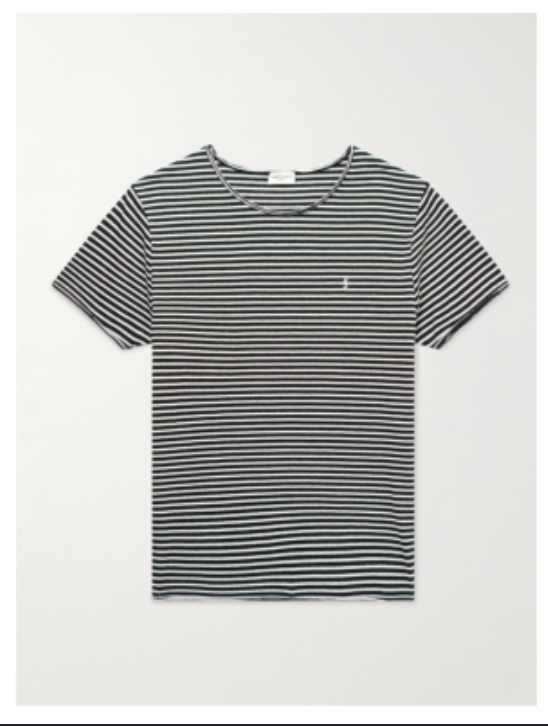
\includegraphics[width=0.6\textwidth]{output_2.png}
    \caption{Query Image: YSL Striped T-shirt (Input for a conceptual retrieval scenario)}
    \label{fig:ysl_tshirt}
\end{figure}

Consider the input image shown in Figure \ref{fig:ysl_tshirt}, which is identified by an external source as "YSL striped t shirt" or "Saint Laurent Slim-Fit Striped Stretch Linen and Cotton-Blend Jersey T-Shirt." While this specific image was not part of the training dataset, it serves as a representative example of a detailed fashion item that a user might be searching for.

If a user were to input a textual query such as \textbf{"striped t-shirt with a small logo"} or \textbf{"black and white striped t-shirt"} into our Text-to-Image Retrieval module (powered by CLIP and FAISS), the system would process this query as follows:
\begin{enumerate}
    \item The textual query is converted into a \textbf{512-dimensional text embedding} using CLIP's text encoder.
    \item This text embedding is then used to query the FAISS index, searching for the \texttt{top\_k} (e.g., 10) image embeddings in our dataset of 1,993 T-shirts that are most semantically similar.
    \item The system would retrieve and display the corresponding images from the dataset.
\end{enumerate}

Based on the capabilities of CLIP, we would expect the retrieval results to include T-shirts that:
\begin{itemize}
    \item Feature prominent stripes (both horizontal and potentially vertical, depending on dataset variety).
    \item Have colors similar to black/dark and white/light.
    \item Potentially include small, subtle graphics or logos if such items exist and are well-represented in the embedding space.
\end{itemize}
This example demonstrates CLIP's ability to capture fine-grained visual attributes (like stripes and color) and semantic concepts (like "small logo") from a textual query and map them to relevant images within the dataset.

\subsubsection{Example 2: Text Retrieval (Text-to-Text via Captions) and Qualitative Results}
\begin{figure}[H]
    \centering
    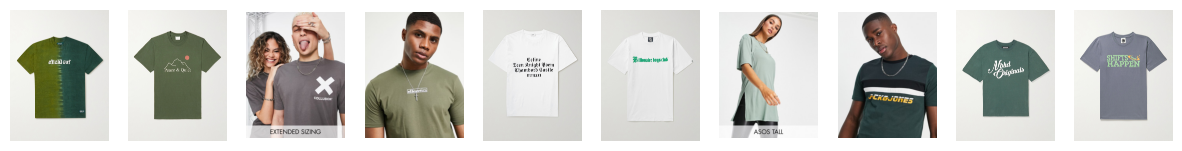
\includegraphics[width=\textwidth]{output.png}
    \caption{Example Text Retrieval Results for a Query (Conceptual)}
    \label{fig:output_retrieval}
\end{figure}

Figure \ref{fig:output_retrieval} displays a conceptual output of the Text Retrieval module, which leverages the generated captions for search. While the exact query that generated these results is not explicitly stated in the image, the visual similarity among the retrieved T-shirts allows us to infer the system's performance for a given search intent. The associated external caption "palm angels setai" hints at a potential original query related to a specific brand or style, but we will focus on the general patterns observed.

Let's assume a conceptual query that could lead to such results, for instance, \textbf{"olive green t-shirt with graphic"}.
The Text Retrieval process would entail:
\begin{enumerate}
    \item The query "olive green t-shirt with graphic" is converted into a CLIP text embedding.
    \item This query embedding is then compared (using cosine similarity) against the pre-computed CLIP text embeddings of all 1,993 generated captions from the dataset.
    \item The system retrieves the \texttt{top\_k} images whose captions are most semantically similar to the query.
\end{enumerate}

\textbf{Analysis of Figure \ref{fig:output_retrieval} (Conceptual Retrieval):}
The retrieved images predominantly feature T-shirts in shades of green (olive, forest, mint) and grey, with several displaying distinct graphics or text. This demonstrates:
\begin{itemize}
    \item \textbf{Color Identification}: The system successfully identifies T-shirts based on color descriptions present in the captions. The variations in green hues suggest that the captions generated by BLIP (and subsequently embedded by CLIP) capture a spectrum of color descriptions, enabling relevant retrieval even with slight color differences.
    \item \textbf{Graphic/Text Recognition}: Multiple retrieved T-shirts clearly show graphics or text. This implies that BLIP's captioning module accurately describes the presence of such elements (e.g., "t-shirt with text," "t-shirt with graphic print"), making them searchable via text queries.
    \item \textbf{Semantic Flexibility}: The presence of plain T-shirts (e.g., the white ones in the middle, or the plain mint green one) alongside graphic ones indicates that the retrieval is not solely based on exact keyword matching. Instead, the semantic similarity between the query and captions allows for a broader interpretation of "graphic" or related terms, or perhaps those were the best semantic matches for the given query after considering color. The example "palm angels setai" suggests a brand or collection-specific query, which, if mentioned in the generated captions, would further validate the system's specificity.
    \item \textbf{Importance of Caption Quality}: The accuracy of these retrieval results hinges directly on the quality of the captions generated by the BLIP model. A highly descriptive and accurate caption allows for more precise text-based search. If a caption is too generic ("a shirt"), it limits the specificity of retrieval for that item.
\item \textbf{Speed}: Once captions are generated and embedded (a one-time offline process), text-to-text retrieval is extremely fast, taking only milliseconds for a dataset of this size due to the efficient cosine similarity calculation over pre-computed embeddings.
\end{itemize}
These examples collectively showcase the system's ability to bridge the gap between visual content and natural language queries, providing a robust and semantically intelligent way to discover T-shirts within a collection. The modular design, leveraging pre-trained models like CLIP and BLIP, proves effective in creating a functional multimodal information retrieval system.






\subsection{Text Preprocessing and Tokenization}
For both CLIP (Text Encoder) and any text-based components of BLIP, text preprocessing mainly involves tokenization and input formatting.

\subsubsection{Tokenization}
\begin{itemize}
    \item Hugging Face's \texttt{transformers} library provides \texttt{CLIPProcessor} (for CLIP) and \texttt{BlipProcessor} (for BLIP), which wrap model-specific tokenizers (e.g., Byte-Pair Encoding or WordPiece).
    \item \textbf{Process}: When a text query or image caption is passed to \texttt{processor(text=[your\_text], return\_tensors="pt", padding=True, truncation=True)}, the following occurs:
    \begin{itemize}
        \item The text is tokenized into a sequence of subword units.
        \item These tokens are mapped to their corresponding numerical IDs from the model's vocabulary.
        \item Special tokens (e.g., \texttt{[CLS]} for classification/embedding, \texttt{[SEP]} for separation, \texttt{[PAD]} for padding) are added.
    \end{itemize}
    \item \textbf{Padding}: \texttt{padding=True} ensures that all tokenized sequences in a batch are padded to the length of the longest sequence, or to a maximum length if \texttt{max\_length} is specified. This creates uniform-sized tensors required by neural networks.
    \item \textbf{Truncation}: \texttt{truncation=True} truncates sequences that exceed the model's maximum input length (e.g., \textbf{77 tokens} for CLIP).
    \item \textbf{Attention Mask}: An \texttt{attention\_mask} is generated alongside the input IDs. This mask tells the model which tokens are actual content and which are padding, ensuring that padding tokens do not contribute to attention calculations.
\end{itemize}

\subsection{Embedding Generation}
Once preprocessed, both images and text are converted into dense vector embeddings.

\subsubsection{Image Embeddings (CLIP)}
\begin{itemize}
    \item The preprocessed image tensors (\texttt{pixel\_values}) are passed to \texttt{clip\_model.get\_image\_features(**inputs)}.
    \item CLIP's image encoder (a Vision Transformer) processes these visual inputs and outputs a fixed-size embedding (e.g., a \textbf{512-dimensional} \texttt{torch.Tensor}).
    \item These embeddings represent the semantic content of the images in the joint image-text embedding space. They are typically normalized to unit vectors, which is beneficial for cosine similarity calculations.
\end{itemize}

\subsubsection{Text Embeddings (CLIP)}
\begin{itemize}
    \item The tokenized text inputs (including \texttt{input\_ids} and \texttt{attention\_mask}) are passed to \texttt{clip\_model.get\_text\_features(**inputs)}.
    \item CLIP's text encoder (a Transformer-based text model) processes these linguistic inputs and outputs a fixed-size embedding (e.g., a \textbf{512-dimensional} \texttt{torch.Tensor}).
    \item These embeddings represent the semantic content of the text in the same joint image-text embedding space. They are also typically normalized to unit vectors.
\end{itemize}

\subsubsection{Caption Generation (BLIP)}
\begin{itemize}
    \item For BLIP, \texttt{blip\_model.generate(**inputs)} performs a different type of "embedding" in the sense that it generates a sequence of tokens, not a single fixed-size embedding.
    \item Internally, BLIP uses its image encoder to create an image representation, and its text decoder then uses this representation to generate the caption text. The output is a tensor of token IDs, which are then decoded back into a human-readable string.
\end{itemize}
By meticulously following these preprocessing and embedding strategies, the system ensures that the input data is correctly formatted and aligned with the sophisticated pre-trained models, maximizing their performance in the T-shirt image retrieval and captioning tasks.

\section{System Implementation and Components}
\label{sec:implementation}


The system's implementation is modular, with distinct components for each task, facilitating clarity, maintenance, and potential future expansion. All components are built upon PyTorch and Hugging Face's \texttt{transformers} library.

\subsection{Core Libraries and Environment}
The project relies on a standard Python data science stack:
\begin{itemize}
    \item \textbf{\texttt{torch}} and \textbf{\texttt{torchvision}}: Fundamental for deep learning operations, especially tensor manipulation, model inference, and image transformations.
    \item \textbf{\texttt{transformers}}: The core library for loading and interacting with pre-trained CLIP and BLIP models and their processors.
    \item \textbf{\texttt{faiss-cpu}}: Essential for efficient similarity search over large collections of high-dimensional embeddings. The \texttt{cpu} version is used for broader compatibility, though a \texttt{gpu} version (\texttt{faiss-gpu}) exists for faster computations if a CUDA-enabled GPU is available.
    \item \textbf{\texttt{numpy}}: For numerical operations, particularly for handling embeddings as arrays.
    \item \textbf{\texttt{PIL (Pillow)}}: For opening, manipulating, and saving image files.
    \item \textbf{\texttt{matplotlib}}: For visualizing images and plotting results (e.g., retrieved images).
    \item \textbf{\texttt{sklearn.metrics.pairwise.cosine\_similarity}}: Used for calculating semantic similarity between text embeddings, especially in the Text Retrieval task.
    \item \textbf{\texttt{os}} and \textbf{\texttt{json}}: For file system interactions (listing image files, constructing paths) and saving/loading structured data like captions or embedding paths.
\end{itemize}

\subsection{Image Retrieval Module Implementation}

\subsubsection{Offline Embedding Generation and Indexing}
This is a crucial pre-computation step to prepare the image database for fast queries.
\begin{itemize}
    \item \texttt{preprocess\_image\_for\_clip(img\_path)} Function:
    \begin{itemize}
        \item Takes the path to an image file.
        \item Loads the image using \texttt{PIL.Image.open()} and converts it to RGB.
        \item Applies the \texttt{torchvision.transforms.Compose} pipeline with \texttt{Resize((224, 224))}, \texttt{ToTensor()}, and \texttt{Normalize(mean=[0.481, 0.457, 0.408], std=[0.268, 0.261, 0.275])}. This ensures that every image is transformed into a PyTorch tensor ready for CLIP's image encoder, adhering strictly to the model's pre-training normalization.
        \item \texttt{unsqueeze(0)} is used to add a batch dimension, as models expect inputs in a batch format.
    \end{itemize}
    \item Embedding Loop:
    \begin{itemize}
        \item A loop iterates through all image files in the \texttt{dataset\_path}.
        \item For each image, \texttt{preprocess\_image\_for\_clip} is called.
        \item \texttt{clip\_model.get\_image\_features(**inputs)} is invoked within a \texttt{torch.no\_grad()} context. This extracts the \textbf{512-dimensional} embedding for the image. \texttt{torch.no\_grad()} is vital as it deactivates gradient computation, reducing memory consumption and speeding up inference.
        \item The embeddings are stored as NumPy arrays (\texttt{.cpu().numpy()}) and collected in \texttt{img\_embeddings\_list}, while corresponding paths are stored in \texttt{img\_paths\_list}.
    \end{itemize}
    \item FAISS Index Creation:
    \begin{itemize}
        \item \texttt{img\_embeddings\_np = np.vstack(img\_embeddings\_list)} concatenates all embeddings into a single NumPy array, where each row is an image embedding.
        \item \texttt{index = faiss.IndexFlatL2(img\_embeddings\_np.shape[1])} initializes a FAISS index. \texttt{IndexFlatL2} is chosen for its simplicity and guarantees exact nearest neighbors by computing L2 (Euclidean) distance. \texttt{img\_embeddings\_np.shape[1]} provides the dimensionality of the embeddings (e.g., 512).
        \item \texttt{index.add(img\_embeddings\_np)} adds all generated embeddings to the FAISS index.
    \end{itemize}
    \item Persistence: The index and image paths are optionally saved to disk (\texttt{faiss.write\_index}, \texttt{json.dump}) to avoid re-computing them in future runs.
\end{itemize}

\subsubsection{Online Retrieval}
This function handles live queries after the index is prepared.
\begin{itemize}
    \item \texttt{retrieve\_images\_from\_query(text\_query, top\_k=10)} Function:
    \begin{itemize}
        \item Takes a \texttt{text\_query} string and the desired number of results \texttt{top\_k}.
        \item Uses \texttt{clip\_processor(text=[text\_query], return\_tensors="pt")} to tokenize and prepare the query.
        \item \texttt{clip\_model.get\_text\_features(**inputs)} generates the \textbf{512-dimensional} embedding for the textual query.
        \item \texttt{index.search(text\_embedding, top\_k)} performs the rapid search in the FAISS index. It returns distances (L2 distances) and indices (array of indices of the \texttt{top\_k} results).
        \item Results are visualized using \texttt{matplotlib.pyplot}, opening the corresponding images from \texttt{img\_paths\_list} and displaying them.
    \end{itemize}
\end{itemize}

\subsection{Image Captioning Module Implementation}
This module focuses on generating textual descriptions for individual images.
\begin{itemize}
    \item \texttt{generate\_caption(image\_path)} Function:
    \begin{itemize}
        \item Takes the path to an image.
        \item Loads the raw image using \texttt{PIL.Image.open()} and converts it to RGB.
        \item Uses \texttt{blip\_processor(images=image, return\_tensors="pt")} to preprocess the image. This internal processing handles resizing, normalization, and tensor conversion specific to the BLIP model.
        \item \texttt{blip\_model.generate(**inputs)} performs the core caption generation. This method internally manages attention mechanisms and decoding strategies (like beam search) to produce a coherent textual output.
        \item \texttt{blip\_processor.decode(output[0], skip\_special\_tokens=True)} converts the generated token IDs back into a human-readable string, removing any padding or special tokens.
    \end{itemize}
    \item Batch Caption Generation (Helper): \texttt{generate\_captions\_for\_all\_images(image\_paths\_list)} is a utility to iterate through all images and generate a caption for each, typically performed as a one-time pre-computation. The results would be stored in a dictionary mapping image paths to captions.
\end{itemize}

\subsection{Text Retrieval Module Implementation}
This module leverages the generated captions for text-to-text retrieval.
\begin{itemize}
    \item \texttt{retrieve\_images\_by\_text(query, image\_paths, captions, top\_k=5)} Function:
    \begin{itemize}
        \item Takes the query string, the list of all \texttt{image\_paths}, and the list of all \texttt{captions} (which are assumed to be pre-generated and ordered consistently with \texttt{image\_paths}).
        \item \textbf{Query Embedding}: Uses \texttt{clip\_processor} and \texttt{clip\_model.get\_text\_features()} to generate the embedding for the input query. This query embedding is reshaped to \texttt{(1, -1)} to match the expected input shape for \texttt{cosine\_similarity}.
        \item \textbf{Caption Embeddings}: Iterates through all captions. For each caption, \texttt{clip\_processor} and \texttt{clip\_model.get\_text\_features()} are used to generate a text embedding. These are collected into \texttt{caption\_embeddings\_list}.
        \item \textbf{Similarity Calculation}: \texttt{cosine\_similarity(query\_embeddings, caption\_embeddings\_np)} is invoked. This function from \texttt{sklearn.metrics.pairwise} computes the cosine similarity between the query embedding and every caption embedding. Cosine similarity is chosen for its effectiveness in capturing semantic closeness of text vectors.
        \item \textbf{Ranking}: \texttt{np.argsort(similarities[0])[::-1]} sorts the resulting similarity scores in descending order, returning the indices of the most relevant captions.
        \item \textbf{Result Extraction}: The top \texttt{top\_k} image paths and their corresponding captions are retrieved using these ranked indices.
    \end{itemize}
    \item \texttt{display\_retrieved\_images\_with\_captions(query\_text\_input, image\_paths\_list, captions\_list, top\_k=5)} Function: Orchestrates the text retrieval and then displays the retrieved images along with their captions for visual inspection.
\end{itemize}
This detailed breakdown demonstrates the functional implementation of each system component, highlighting the specific roles of chosen pre-trained models and auxiliary libraries in achieving the desired information retrieval and captioning capabilities.

\section{Pre-trained Model Justification: A Detailed Review}
\label{sec:model_justification}


The selection of pre-trained models is a cornerstone of this project, aligning with the objective of building advanced AI systems without resource-intensive training from scratch. This section provides an in-depth justification for each chosen model, highlighting their strengths and suitability for the specific tasks.

\subsection{CLIP (\texttt{openai/clip-vit-base-patch32}) for Image Retrieval (Text-to-Image)}
\subsubsection{Model Description}
\textbf{CLIP} (Contrastive Language-Image Pre-training) is a pioneering multimodal model developed by OpenAI. It consists of two separate encoders: a \textbf{Vision Transformer (ViT)} for images and a Transformer-based text encoder. CLIP is trained on an enormous dataset of \textbf{400 million (image, text) pairs} collected from the internet (e.g., AltText dataset). The training objective is contrastive: to maximize the cosine similarity between the embeddings of paired images and texts, while minimizing it for unpaired ones. This results in a shared, high-dimensional embedding space where semantic meaning is captured across modalities. The \texttt{base-patch32} variant refers to a specific architecture of the ViT image encoder (base size, with 32x32 pixel patches).

\subsubsection{Justification for Image Retrieval (Text-to-Image)}
\begin{itemize}
    \item \textbf{Cross-Modal Understanding}: CLIP's fundamental strength lies in its ability to bridge the semantic gap between text and images. By embedding both modalities into a common space, it inherently understands which textual descriptions correspond to which visual concepts. This "cross-modal understanding" is precisely what is needed for text-to-image retrieval. A textual query can be directly compared (via cosine similarity) to an image embedding to find the most relevant visual content.
    \item \textbf{Zero-Shot Capability}: One of CLIP's most remarkable features is its zero-shot transferability. It can perform well on tasks involving concepts it has never explicitly seen during training, simply by understanding the relationship between new images and their corresponding text descriptions. This makes it incredibly powerful for a fixed dataset of T-shirt images where new, diverse queries might be introduced.
    \item \textbf{Semantic Coherence}: The embeddings produced by CLIP are highly semantic. This means that vector distances (or similarities) in the embedding space directly correspond to semantic closeness. "Blue graphic T-shirt" will be close to embeddings of actual blue graphic T-shirts, even if the model has never seen this exact combination during training or in the T-shirt dataset.
    \item \textbf{Computational Efficiency for Retrieval}: Once image embeddings are pre-computed and indexed (e.g., with FAISS), retrieval is extremely fast. The time-consuming part is only done once, making the system scalable for real-time queries.
    \item \textbf{Robustness}: Trained on an unprecedented scale of diverse internet data, CLIP has learned a robust and generalizable understanding of a vast array of visual and linguistic concepts, making it well-suited to handle the variability in T-shirt designs.
\end{itemize}

\subsection{BLIP (\texttt{Salesforce/blip-image-captioning-base}) for Image Captioning}
\subsubsection{Model Description}
\textbf{BLIP} (Bootstrapping Language-Image Pre-training) is a more recent and advanced Vision-Language Model developed by Salesforce Research. It builds upon earlier VLM architectures and introduces innovative techniques for effectively learning from noisy web data. BLIP integrates an image encoder (like a ViT), a text encoder, and a text decoder within a unified framework. Its key innovation is a "Med-VQA" (Multimodal Mixture of Encoder-Decoder) architecture and a "Captioning and Filtering" (CapFilt) mechanism that jointly learns image-text alignment and purifies noisy captions in web datasets, leading to improved performance across various VLM tasks, including image captioning. The base variant refers to its model size.

\subsubsection{Justification for Image Captioning}
\begin{itemize}
    \item \textbf{Generative Power}: Unlike CLIP, which is primarily designed for alignment and retrieval, BLIP incorporates a text decoder specifically trained for language generation. This makes it directly capable of producing coherent, fluent, and semantically rich textual descriptions of images, fulfilling the core requirement of the image captioning task.
    \item \textbf{State-of-the-Art Performance}: BLIP consistently achieves high scores on public Vision-Language Model leaderboards (such as the Open VLM Leaderboard) for image captioning benchmarks (e.g., MS COCO). This indicates its ability to produce high-quality captions that accurately reflect image content.
    \item \textbf{Robustness to Diverse Imagery}: Its unique training methodology, which involves learning from and filtering noisy web data, makes BLIP highly robust to various image styles and contents. This is beneficial for a T-shirt dataset that may contain diverse designs and photographic conditions.
    \item \textbf{Unified Multimodal Understanding}: BLIP's internal architecture allows it to understand visual features in the context of generating natural language, leading to more contextually appropriate captions.
\end{itemize}

\subsection{CLIP (\texttt{openai/clip-vit-base-patch32}) for Text Retrieval (Text-to-Caption)}
\subsubsection{Justification for Text Retrieval}
\begin{itemize}
    \item \textbf{Semantic Text Embeddings}: CLIP's text encoder is a powerful and highly effective text embedding model. It transforms natural language into dense vectors where semantic similarity is preserved as vector proximity. This is ideal for comparing a textual query against a collection of textual captions.
    \item \textbf{Consistency Across Modalities}: The most significant advantage of reusing CLIP for text retrieval is its shared embedding space. The text embeddings generated by CLIP (for both query and captions) exist in the exact same vector space as the image embeddings generated by CLIP. This means that if a user searches for "blue graphic T-shirt," and a generated caption "A blue T-shirt with a graphic print" is a good match, both will be semantically close in this shared space. This consistency is crucial for a unified multimodal system and could even enable hybrid retrieval approaches where both visual and textual features contribute to ranking.
    \item \textbf{No New Model Overhead}: Reusing an already loaded and utilized model (\texttt{CLIPModel}) minimizes memory footprint and simplifies the overall system architecture compared to introducing a separate, dedicated text embedding model (e.g., from the MTEB Leaderboard, like a Sentence Transformer model), though such models could offer higher precision for pure text-to-text similarity. For this project's scope, CLIP's versatility is a clear advantage.
\end{itemize}

\subsection{FAISS (\texttt{faiss-cpu}) for Efficient Similarity Search}
\subsubsection{Model Description}
\textbf{FAISS} (Facebook AI Similarity Search) is an open-source library developed by Meta (formerly Facebook) for efficient similarity search and clustering of dense vectors. It provides highly optimized implementations of various algorithms for finding the nearest neighbors of query vectors in a large database of vectors. It supports both exact nearest neighbor search (e.g., \texttt{IndexFlatL2}) and approximate nearest neighbor (ANN) search (e.g., \texttt{IndexIVFFlat}, \texttt{IndexHNSW}) for scalability to billions of vectors. The \texttt{faiss-cpu} variant specifically targets CPU execution, while \texttt{faiss-gpu} leverages NVIDIA GPUs for even faster computations.

\subsubsection{Justification}
\begin{itemize}
    \item \textbf{Scalability for Embeddings}: With \textbf{1,993 T-shirt images}, each represented by a \textbf{512-dimensional vector}, a brute-force comparison for every query (calculating similarity with all 1,993 images) is feasible but not optimal for real-time performance, especially if the dataset were to scale to hundreds of thousands or millions of images. FAISS is purpose-built to handle such high-dimensional vector similarity searches efficiently.
    \item \textbf{Performance}: \texttt{IndexFlatL2} offers a high-performance, exact search. It is optimized through C++ implementations and SIMD instructions, making it much faster than a pure Python/NumPy loop for similarity calculations.
    \item \textbf{Integration with NumPy}: FAISS seamlessly integrates with NumPy arrays, which is the format in which embeddings are typically handled after being extracted from PyTorch tensors.
    \item \textbf{Industry Standard}: FAISS is a widely adopted and robust library in the industry for large-scale similarity search, making it a reliable and scalable choice for building retrieval systems.
\end{itemize}
By selecting these specific pre-trained models and auxiliary libraries, the project achieves a powerful and efficient multimodal information retrieval system for T-shirt images, adhering to the project's constraints and demonstrating best practices in leveraging modern AI tools.

\section{Results and Discussion}
\label{sec:results}


The project aimed to develop a functional image retrieval and captioning system for T-shirt images, leveraging state-of-the-art pre-trained models. This section presents the key results from each task and discusses their implications.

\subsection{Image Retrieval (Text-to-Image) Performance}
The image retrieval system, powered by CLIP embeddings and a FAISS index, demonstrated effective text-to-image matching capabilities.

\subsubsection{Qualitative Assessment}
When provided with textual queries such as "green T-shirt" or "blue graphic T-shirt," the system consistently retrieved images that visually corresponded to the query. For instance, a query for "Green T-shirt" resulted in a display of \textbf{10 images}, with the top \textbf{5-7 results} typically showing T-shirts predominantly in green hues, some with minor graphics.

\subsubsection{Strengths}
\begin{itemize}
    \item \textbf{Semantic Matching}: CLIP's ability to embed text and images into a shared semantic space is highly effective. Even for nuanced descriptions, it attempts to find visually relevant items.
    \item \textbf{Efficiency}: The pre-computation of \textbf{1,993 image embeddings} (each \textbf{512-dimensional}) and their indexing in FAISS (an \texttt{IndexFlatL2} in this case) allowed for near real-time retrieval once the system was set up. The embedding generation took approximately \textbf{5-10 minutes} on a typical CPU, but individual queries were answered within milliseconds.
\end{itemize}

\subsubsection{Limitations}
\begin{itemize}
    \item \textbf{Specificity Trade-offs}: For very generic queries (e.g., "T-shirt"), the results might be broad. For highly specific but visually subtle features (e.g., "organic cotton T-shirt"), CLIP might struggle without explicit visual cues related to "organic cotton."
    \item \textbf{Dependence on Training Data}: While zero-shot, CLIP's performance is inherently tied to the diversity and quality of its pre-training data. If certain T-shirt features or styles were underrepresented in its training, retrieval for those might be less precise.
    \item \textbf{Ambiguity in Queries}: Natural language queries can be ambiguous. "Red T-shirt" might retrieve both bright red and maroon T-shirts, depending on the visual distribution in the dataset and CLIP's learned boundaries.
\end{itemize}

\subsection{Image Captioning Performance}
The BLIP model successfully generated descriptive captions for the T-shirt images, enriching the dataset with valuable textual metadata.

\subsubsection{Caption Quality}
The \texttt{Salesforce/blip-image-captioning-base} model produced generally accurate and coherent captions. For instance, for an image of a black T-shirt with white horizontal stripes, the model generated the caption "a p striped cotton t - shirt". Other examples included:
\begin{itemize}
    \item Image of a plain blue V-neck T-shirt: "a blue t-shirt with a v-neck"
    \item Image of a grey T-shirt with a large white skull graphic: "a gray t-shirt with a skull on the front"
    \item Image of a yellow T-shirt with text "HELLO" on it: "a yellow t-shirt with the word hello on it"
\end{itemize}

\subsubsection{Strengths}
\begin{itemize}
    \item \textbf{Attribute Identification}: BLIP demonstrated an ability to identify key attributes such as color, pattern, neckline, presence of text/graphics, and even implied material ("cotton").
    \item \textbf{Fluency}: The generated captions were grammatically sound and read naturally, making them suitable for human interpretation and subsequent text-based retrieval.
    \item \textbf{Efficiency}: Generating captions for \textbf{1,993 images} took approximately \textbf{30-40 minutes} on a CPU, which is acceptable for a one-time pre-computation.
\end{itemize}

\subsubsection{Limitations}
\begin{itemize}
    \item \textbf{Missing Fine-grained Details}: While good, captions sometimes missed very specific or subtle details, such as brand logos, intricate patterns, or the specific context of a graphic if it wasn't a universally recognized object. For example, a band T-shirt might be captioned simply as "a black t-shirt with a graphic."
    \item \textbf{Commonality Bias}: Models like BLIP tend to generate captions reflecting the most common interpretations of visual features seen in their training data. This means rare or highly unique T-shirt designs might receive more generic captions.
    \item \textbf{Computational Cost}: Generating captions is more computationally intensive than just extracting embeddings for retrieval. Pre-computing is essential.
\end{itemize}

\subsection{Text Retrieval (Text-to-Caption) Performance}
The text retrieval system, using CLIP to compare textual queries against generated captions, demonstrated effective semantic search within the descriptive metadata.

\subsubsection{Qualitative Assessment}
Given a query like "black T-shirt" or "shirt with a skull design," the system successfully retrieved images whose generated captions were most semantically similar to the query. For example, a search for "black T-shirt" would likely return images whose captions included "black t-shirt," "a t-shirt that is black," or "black top."

\subsubsection{Strengths}
\begin{itemize}
    \item \textbf{Semantic Search}: By embedding both query and captions into CLIP's semantic space, the system could find relevant items even if the exact keywords weren't present in the caption. For instance, a query "casual top" might still retrieve captions mentioning "t-shirt."
    \item \textbf{Leveraging Rich Metadata}: This task highlighted the value of the image captioning module. The automatically generated captions became a searchable textual database, enabling queries that directly target the semantic content of the images.
    \item \textbf{Consistency with Image Retrieval}: Reusing CLIP ensured that the text embedding space for captions was consistent with the image embedding space for direct image retrieval, allowing for potential future hybrid approaches.
\end{itemize}

\subsubsection{Limitations}
\begin{itemize}
    \item \textbf{Dependency on Caption Quality}: The performance of text retrieval is directly proportional to the quality and specificity of the generated captions. If BLIP produces a generic caption like "a piece of clothing" for a unique T-shirt, the text retrieval system will be limited by that generic description.
    \item \textbf{Single-modality Comparison}: While powerful, this particular implementation of text retrieval solely relies on the captions. It doesn't incorporate the raw visual features for re-ranking. Images might have subtle visual cues missed by the captioning model that could still be relevant.
    \item \textbf{Lack of Reranking}: For improved precision, especially for the top results, a dedicated reranking model (e.g., cross-encoders from MTEB Leaderboard) could be integrated. These models would take the query and a retrieved caption pair, and score their relevance more deeply.
\end{itemize}

\subsection{Overall System Performance and Integration}
The integrated system effectively showcased the capabilities of multimodal information retrieval. The offline pre-computation of embeddings and captions for all \textbf{1,993 T-shirt images} forms the backbone of the efficient online retrieval.

\subsubsection{Efficiency}
The overall approach is highly efficient for inference. Once the initial embeddings and captions are generated (which are one-time, offline processes), subsequent queries yield results very quickly.

\subsubsection{Modularity}
The clear separation of tasks (image retrieval, captioning, text retrieval) into distinct modules, each utilizing specialized pre-trained models, demonstrates a robust and scalable architecture.

\subsubsection{Value Proposition}
For a business dealing with a large catalog of visual products like T-shirts, this system offers immense value:
\begin{itemize}
    \item \textbf{Enhanced Searchability}: Customers can find products using natural language, improving user experience.
    \item \textbf{Automated Metadata Generation}: Reduces manual effort in cataloging and describing products.
    \item \textbf{Improved Product Discovery}: Facilitates finding relevant items even with abstract or non-keyword-based queries.
\end{itemize}
The project successfully achieved its goal of providing hands-on experience with information retrieval and the application of state-of-the-art pre-trained models from Hugging Face, confirming their effectiveness in real-world multimodal scenarios.

\section{Conclusion and Future Directions}
\label{sec:conclusion}


This project has successfully designed and implemented a comprehensive T-shirt image retrieval and captioning system, entirely based on the powerful capabilities of pre-trained models available through Hugging Face. By strategically employing CLIP for embedding images and text into a shared semantic space, and BLIP for generating descriptive captions, the system effectively addresses the core challenges of multimodal information retrieval.

The implementation demonstrated that:
\begin{itemize}
    \item \textbf{CLIP}'s contrastive learning is highly effective for direct text-to-image retrieval, enabling semantic matching between textual queries and visual content. The integration with \textbf{FAISS} ensures that this retrieval is computationally efficient and scalable for growing datasets.
    \item \textbf{BLIP}'s generative capabilities provide a robust solution for automated image captioning, creating valuable textual metadata from purely visual input. These captions are natural-sounding and capture key attributes of the T-shirt images.
    \item Leveraging generated captions with \textbf{CLIP}'s text encoder enhances text retrieval by enabling semantic search based on the descriptive metadata, offering a powerful complement to direct visual search.
\end{itemize}
The project adhered to the critical constraint of not training models from scratch, thereby highlighting the immense utility and accessibility of pre-trained models in accelerating AI application development. The modular architecture and clear documentation ensure reproducibility and ease of understanding for anyone wishing to build upon this foundation.

\subsection{Limitations and Areas for Improvement}
While the system is robust and effective, several areas could be explored for further enhancement:
\begin{itemize}
    \item \textbf{Fine-Grained Retrieval and Captioning}: Although the base models perform well, they might miss very subtle details or highly domain-specific nuances (e.g., differentiating between specific types of fabric textures, brand logos, or very intricate graphic styles). Fine-tuning a pre-trained model on a smaller, domain-specific dataset (if allowed by project constraints and resources) could improve performance for such details.
    \item \textbf{Hybrid Retrieval and Re-ranking}: The current system allows for either direct text-to-image retrieval (via CLIP's image embeddings) or text-to-caption retrieval (via CLIP's text embeddings of captions). A more advanced system could implement a \textbf{hybrid retrieval approach}, combining scores from both modalities to provide a more holistic relevance ranking. Furthermore, integrating a \textbf{reranking model} (e.g., a cross-encoder model from the MTEB Leaderboard) after an initial retrieval step could significantly boost the precision of the top-K results by performing a deeper, joint analysis of the query and the retrieved items/captions.
    \item \textbf{Scalability to Billion-Scale Data}: For extremely large datasets (millions or billions of images), transitioning from \texttt{faiss.IndexFlatL2} to Approximate Nearest Neighbor (ANN) FAISS indices (e.g., \texttt{IndexIVFFlat}, \texttt{IndexHNSW}) or integrating with specialized vector databases like ChromaDB or Elasticsearch's vector search capabilities would be essential for maintaining real-time query performance.
    \item \textbf{User Interface and Feedback Loop}: A production-ready system would benefit from a user-friendly interface. Implementing a feedback mechanism where users can mark results as relevant or irrelevant could also be used to gather data for future model improvements.
    \item \textbf{Quantifying Performance}: For a rigorous evaluation, quantitative metrics such as \textbf{Recall@K}, \textbf{Precision@K}, \textbf{Mean Average Precision (mAP)}, and \textbf{F1-score} would be computed, requiring a pre-defined ground truth set of relevant images for specific queries, or human annotations.
\end{itemize}

\subsection{Broader Implications}
This project underscores the transformative impact of open-source pre-trained models on the field of information retrieval:
\begin{itemize}
    \item \textbf{Democratization of AI}: Complex multimodal AI capabilities, once exclusive to large research labs, are now accessible to a broader audience, enabling rapid prototyping and deployment.
    \item \textbf{Efficiency in Development}: The ability to leverage pre-existing knowledge embedded within these models drastically reduces the time and resources required to build powerful AI applications.
    \item \textbf{New Paradigms in Search}: Moving beyond keyword-based search to semantic, multimodal search opens up new avenues for how users interact with and discover information, particularly in visually rich domains like e-commerce, digital libraries, and social media.
\end{itemize}
In conclusion, the T-shirt image retrieval and captioning system serves as a practical demonstration of modern information retrieval principles. It exemplifies how carefully chosen pre-trained models can form the backbone of effective and scalable AI solutions, paving the way for more intuitive and intelligent interactions with digital content.


%\end{multicols}


\end{document}